\section{Prior Work Completed\label{introduction:priorWork}}

This project idea of an improved lumpectomy tumor bed marking method was first proposed by the Division Chief for Oncoplastic Surgery at The Ohio State University Comprehensive Cancer Center (OSUCCC), Dr. Roman Skoracki~\cite{RefWorks:RefID:372-krakovskytumor},~\cite{RefWorks:RefID:371-bakhtardesign}.

This project was then adopted bya mechanical engineering senior capstone in 2022 (\hl{Check this date}). It has since been further explored by Adrian Bakhtar, Isaac Einstein, and Zuhaib Jama. The general contributions of each group are summarized below in Table~\ref{tab:introduction:priorWorkCompletedOverview}.

\begin{table}[H]
        \centering
        \caption{Summary of Prior Team and Researcher Contributions}
        \label{tab:introduction:priorWorkCompletedOverview}
        \begin{tabularx}{\textwidth}{>{\raggedright\arraybackslash}p{3cm} X >{\raggedright\arraybackslash}p{3cm}}
                \toprule
                \textbf{Team/Researcher}                                       & \textbf{General Contribution(s)} & \textbf{Time Working on Project} \\
                \midrule
                Senior Capstone Group~\cite{RefWorks:RefID:372-krakovskytumor} &
                - Identified initial pain points and opportunity \newline
                - Evaluated various end-product concepts \newline
                - Selected ideal form factor and developed initial device prototype
                                                                               & 2022                                                                \\
                \addlinespace
                Adrian Bakhtar~\cite{RefWorks:RefID:371-bakhtardesign}         &
                - Continued work started by senior capstone team \newline
                - Worked with stakeholders to refine device design \newline
                - Optimized device geometry, printability, and adhesive capabilities \newline
                - Defended master's thesis and is continuing research through a PhD
                                                                               & 2022 -- Present                                                     \\
                \addlinespace
                Zuhaib Jama~\cite{RefWorks:RefID:384-jamacomputational}        &
                - Evaluated potential stresses experienced by the device via FEM \newline
                - Presented findings at research poster symposium
                                                                               & 2024                                                                \\
                \addlinespace
                Isaac Einstein~\cite{RefWorks:RefID:370-einsteinisaac}         &
                - Evaluated material properties of device base material \newline
                - Presented findings through a research poster symposium and undergraduate thesis
                                                                               & 2023 -- 2024                                                        \\
                \bottomrule
        \end{tabularx}
\end{table}

\subsection{Senior Capstone Work\label{sec:introduction:priorWork:seniorCapstone}}

\subsubsection{Device Requirements\label{sec:introduction:priorWork:seniorCapstone:deviceRequirements}}
Working alongside the OSUCCC including surgeons, radiation oncologists, and dosimetrists, the senior capstone team developed target functional requirements for the device. This is outlined below in Table~\ref{tab:introduction:priorWork:seniorCapstone:targetSpecifications}.

\begin{table}[H]
        \centering
        \caption{Initial Device Target Specifications~\cite{RefWorks:RefID:372-krakovskytumor},~\cite{RefWorks:RefID:371-bakhtardesign}}
        \label{tab:introduction:priorWork:seniorCapstone:targetSpecifications}
        \begin{tabularx}{\textwidth}{
                >{\centering\arraybackslash}p{1.2cm}
                >{\raggedright\arraybackslash}p{3.5cm}
                X
                }
                \toprule
                \textbf{Weight} & \textbf{Specification} & \textbf{Requirement} \\
                \midrule
                1               & Biocompatibility       &
                Follows ISO 10993 \newline
                • Twenty-part protocol FDA testing process                      \\
                \addlinespace
                2               & Sterilizable           &
                Follows ISO 11135 \newline
                • Sterilization of health-care products (Ethylene oxide) \newline
                Packaging follows ISO 11607 \newline
                • Packaging for sterilized material                             \\
                \addlinespace
                3               & Implantation speed     &
                < 3 minutes                                                     \\
                \addlinespace
                4               & Radiodensity           &
                > 0 HU and < 3000 HU (Hounsfield Units)                         \\
                \addlinespace
                5               & Longevity              &
                6 weeks -- 12 months                                            \\
                \addlinespace
                6               & Mechanical Properties  &
                812 -- 4500 kg/m\textsuperscript{3}                             \\
                \addlinespace
                7               & Size/Area              &
                2 -- 7 cm in diameter \newline
                10 -- 150 cm\textsuperscript{2}                                 \\
                \addlinespace
                8               & Cost                   &
                < \$1250                                                        \\
                \bottomrule
        \end{tabularx}
\end{table}

Because the device would eventually be implanted in human patients, biocompatibility and sterilization were given the highest importance. Implantation speed was next based on surgeon feedback~\cite{RefWorks:RefID:372-krakovskytumor}.

It was believed the chances of device adoption by surgeons would decrease if implantation speed was significant~\cite{RefWorks:RefID:372-krakovskytumor}.

Discussions with dosimetrists led the group to select a target Hounsfield Units (HU) of less than 3,000 HU to reduce radiation reflection and provide adequate contrast from breast tissue~\cite{RefWorks:RefID:372-krakovskytumor}.

The longevity of the device was estimated through conversations with OSUCCC based on the range of lumpectomy procedure timelines~\cite{RefWorks:RefID:372-krakovskytumor}.

The mechanical properties were selected to mirror breast tissue based on additional team research~\cite{RefWorks:RefID:372-krakovskytumor}.

Lastly, the size and cost of the device were selected based on research into existing competitor devices~\cite{RefWorks:RefID:372-krakovskytumor}.

\subsubsection{Initial Prototype Development\label{sec:introduction:priorWork:seniorCapstone:initialPrototypeDevelopment}}

\paragraph*{Material Selection\label{sec:introduction:priorWork:seniorCapstone:initialPrototypeDevelopment:materialSelection}}
To adhere with the mechanical properties and biodegradable needs of the device, the capstone team selected Poly(l-lactide-co-$\varepsilon$-caprolactone) (PLCL) as the base material. This is a biodegradable and biocompatible material with an adjustable degredation timeline and mechanical properties. It is composed of two co-polymers: Polylactic acid (PLA) and Polycaprolactone (PCL). The radiopaque agent selected was barium sulfate (BaSO4) based on its extensive clinical trials and current use in digestive marking~\cite{RefWorks:RefID:372-krakovskytumor}.

\paragraph*{Device Form Factor\label{sec:introduction:priorWork:seniorCapstone:initialPrototypeDevelopment:formFactor}}
As shown in Figure~\ref{fig:introduction:initialCapstonePrototype}, the capstone team designed the device in a hemispherical and collapsible form factor. The team created the prototype through melting base materials into a premade mold~\cite{RefWorks:RefID:372-krakovskytumor}.

\paragraph*{Imaging Testing\label{sec:introduction:priorWork:seniorCapstone:initialPrototypeDevelopment:imaginTesting}}

Imaging capabilities and radiopacity of the initial prototype was evaluated by the capstone team to evaluate the desired amount of barium sulfate. This initial testing resulted in excessively bright samples, which illustrated the need to minimal barium sulfate addition~\cite{RefWorks:RefID:372-krakovskytumor}. The capstone team's imaging testing is shown below in Figure~\ref{fig:introduction:capstoneImagingTesting}.

\begin{figure}[h!]
        \centering
        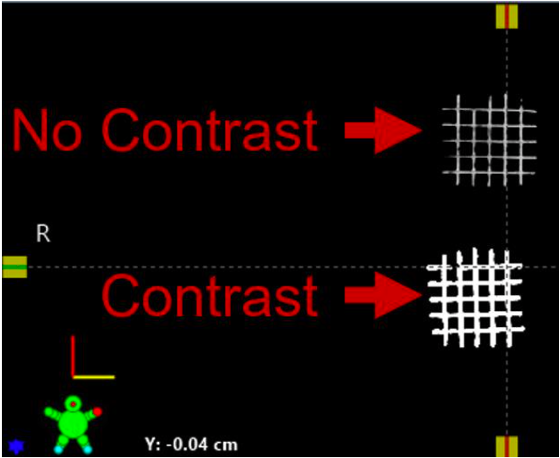
\includegraphics[width=0.8\textwidth]{../figs/introduction/capstone_imaging_testing.png}
        \caption{Initial imaging results from senior capstone team~\cite{RefWorks:RefID:372-krakovskytumor}.}
        \label{fig:introduction:capstoneImagingTesting}
\end{figure}

\subsubsection{Future Work\label{sec:introduction:priorWork:seniorCapstone:futureWork}}

The senior capstone, while making strides in the early development of the device, had areas that could benefit from additional testing. This includes focusing on optimizing the manufacturing process, making the overall mesh thinner, decreasing the amount of barium sulfate embedded, and performing longer-term biodegradability testing.

\subsection{Additional Research Team Work\label{sec:introduction:priorWork:otherTeamWork}}

\subsubsection{Customer Discovery\label{sec:introduction:priorWork:otherTeamWork:customerDiscovery}}

\paragraph*{Stakeholder Interviews\label{sec:introduction:priorWork:otherTeamWork:customerDiscovery:interviews}}

Numerous interviews were conducted throughout the early-stage development of this device to ensure the device was designed with stakeholder needs in mind. These stakeholders and potential end-users included: surgical oncologists, plastic and reconstructive surgeons, and radiation oncologists. As shown in Figure~\ref{fig:ecosystemMap}, an ecosystem map was developed to illustrate how this device may interact with potential stakeholders.

\begin{figure}[h!]
        \centering
        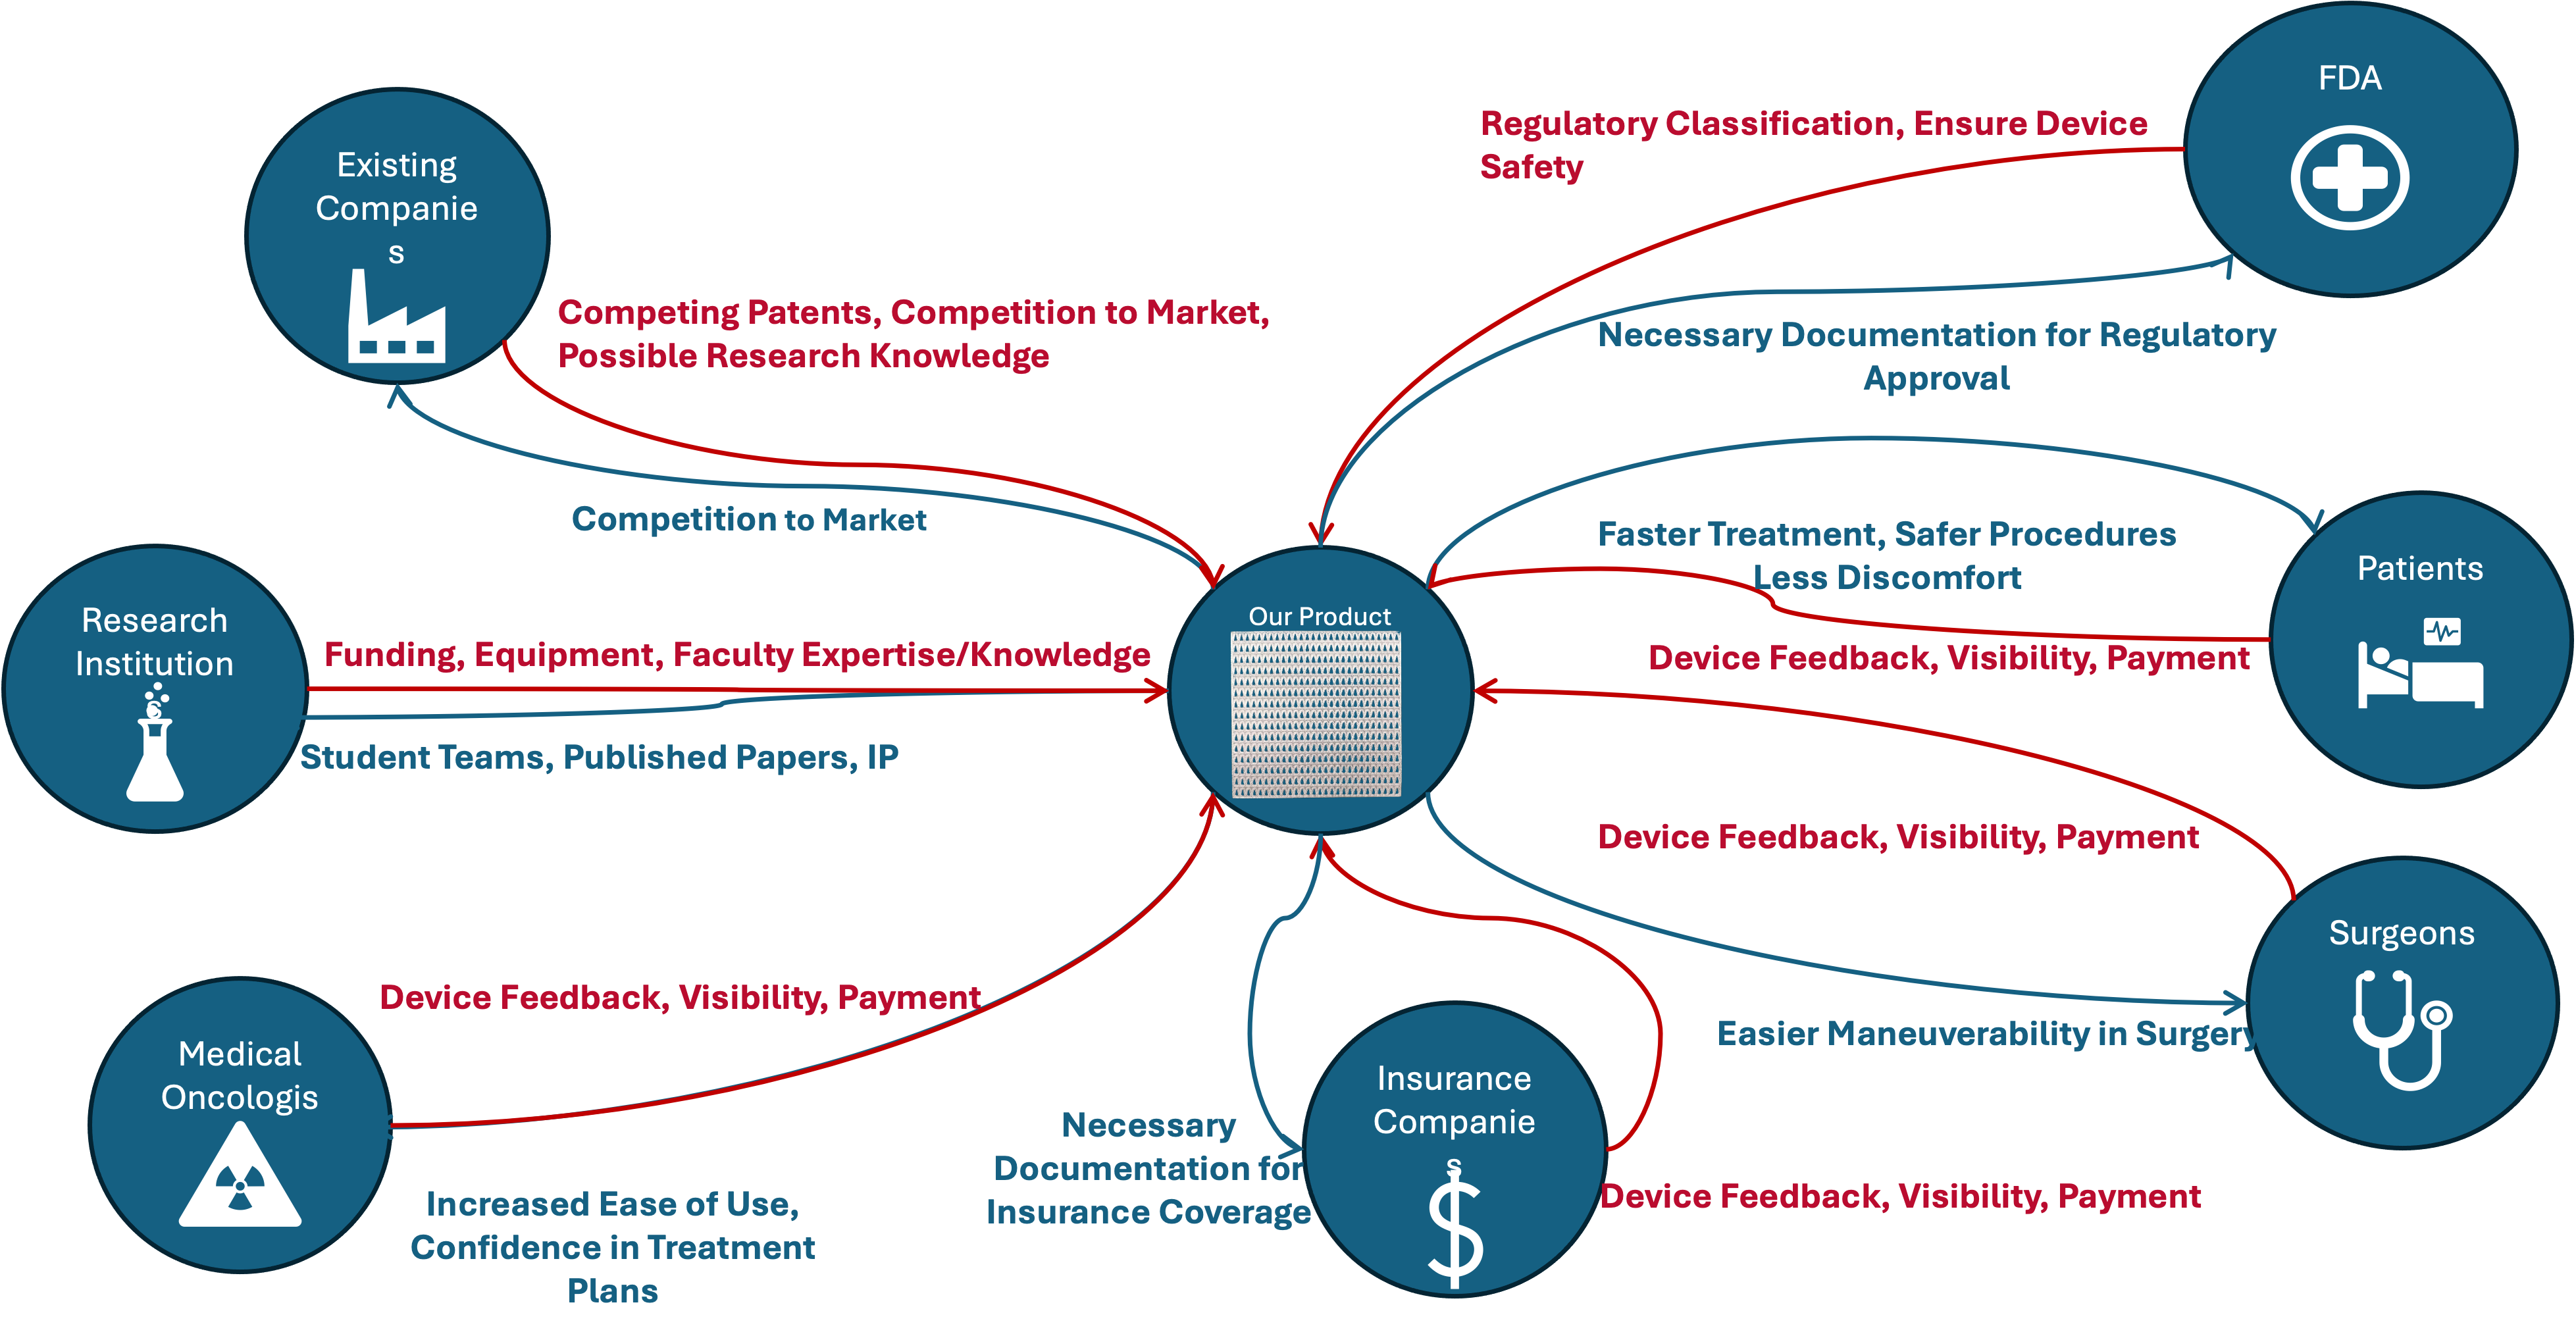
\includegraphics[width=0.8\textwidth]{../figs/introduction/ecosystem_mapping.png}
        \caption{Interactions between this device and potential stakeholders. Stakeholder impact on the device development are shown in red while the device's potential impact on stakeholders is shown in gray~\cite{RefWorks:RefID:386-bakhtarvisualizing}.}
        \label{fig:introduction:ecosystemMap}
\end{figure}

These interviews challenged the team's current device assumptions with topics such as using fiducial markers in surgery, imaging visibility, adoption barriers, and feedback on the current design~\cite{RefWorks:RefID:371-bakhtardesign}.

From these preliminary interviews, various stakeholder key requirements were developed. These key requirements are detailed below in Table~\ref{tab:introduction:priorWork:preliminaryStakeholderInterviewResults}.

\begin{table}[h!]
        \centering
        \caption{Stakeholder Key Requirements From Preliminary Interviews~\cite{RefWorks:RefID:172-2024reexcision}}
        \label{tab:introduction:priorWork:preliminaryStakeholderInterviewResults}
        \begin{tabular}{p{4cm} p{10cm}}
                \hline
                \textbf{Clinician Group}        & \textbf{Key Requirements}       \\
                \hline
                Surgical Oncologists            &
                \vspace{-\baselineskip}\begin{itemize}[leftmargin=*]
                                               \item Flexible and trimmable
                                               \item Easily insertable/fixable
                                               \item Fully resorbable in 6--12 months
                                       \end{itemize}      \\

                Plastic/Reconstructive Surgeons &
                \vspace{-\baselineskip}\begin{itemize}[leftmargin=*]
                                               \item Conformable to tissue
                                               \item Easy to secure and trimmable
                                       \end{itemize}          \\

                Radiation Oncologists           &
                \vspace{-\baselineskip}\begin{itemize}[leftmargin=*]
                                               \item Continuous lumpectomy cavity coverage
                                               \item Stable positioning over time
                                               \item Reliably radiopaque
                                               \item Accurate marking to allow for APBI
                                       \end{itemize} \\
                \hline
        \end{tabular}
\end{table}

\paragraph*{I-Corps\label{sec:introduction:priorWork:otherTeamWork:customerDiscovery:iCorps}}

The research team participated in the NSF Local I-Corps program at Ohio State University. This is a six-week training focused on helping early-stage researchers establish and verify a marketable need for their research as well as prepare them for future commercialization. Through this program, many user interviews were conducted that helped redefine the team's initial assumptions~\cite{RefWorks:RefID:386-bakhtarvisualizing}.

Initially, the team assumed that creating a mesh with patient specific geometry would be helpful and advantageous, point markers are insufficient for accurately marking a tumor margin, and a continuously radiopaque marker would standardize and quicken the therapy planning process~\cite{RefWorks:RefID:386-bakhtarvisualizing}.

Some of these assumptions were validated while others were challenged through this I-Corps training. It was found that rather than patient-specific geometry, thin flexible sheets that could be cut to a patient's tumor during surgery are preferred by surgeons. It was also found that a textured side to the mesh would benefit surgeons and radiation oncologists. Radiation oncologists agreed that fiducial markers alone are an inadequate method of marking tumor margins. Lastly, though radiation oncologists felt this device may not save time when creating treatment plans, they did feel it would greatly improve the accuracy, cost, and number of treatment sessions for each patient~\cite{RefWorks:RefID:386-bakhtarvisualizing}.
\subsubsection{3D Printing Work\label{sec:introduction:priorWork:otherTeamWork:3dPrinting}}

\paragraph*{Optimizing PLCL Printing Parameters\label{sec:introduction:priorWork:otherTeamWork:3dPrinting:plclParameters}}

While development of a custom PLCL 3D printable filament was underway, externally sourced PLCL filament was bought for mechanical testing and improvement of device design. 1.75mm filament was bought from Lattice Medical, a French-based company~\cite{RefWorks:RefID:42-latticemedical}.

Fused deposition modeling (FDM) printing was conducted with this filament (see Section~\ref{chap:literatureReview} [\hl{Update \# after adding 3D printing section}] for additional information on FDM printing).

Necessary printing parameters, including nozzle temperature, bed temperature, layer height, infill density, and print speed, needed to be adjusted and optimized for the Lattice PLCL filament. Multiple line tests and scaled device prints were preformed to manually optimize the printing parameters for this filament. The optimal parameters are shown below in Table~\ref{tab:introduction:priorWork:plclPrintingParameters}~\cite{RefWorks:RefID:371-bakhtardesign}. These tests were conducted using a Prusa i3 MK3 printer.

\begin{table}[h!]
        \centering
        \caption{Optimal Printing Parameters for Lattice PLCL on Prusa i3 MK3 Printer}
        \label{tab:introduction:priorWork:plclPrintingParameters}
        \begin{tabularx}{0.8\textwidth}{
                >{\raggedright\arraybackslash}p{5cm}
                >{\raggedright\arraybackslash}X
                }
                \toprule
                \textbf{Parameter}                  & \textbf{Optimal Value} \\
                \midrule
                First layer print speed             & 20 mm/s                \\
                First layer nozzle temperature      & 180\,\textdegree C     \\
                Subsequent layer nozzle temperature & 190\,\textdegree C     \\
                Bed temperature                     & 30\,\textdegree C      \\
                Infill density                      & 10\%                   \\
                \bottomrule
        \end{tabularx}
\end{table}

\subsubsection{Design of Device\label{sec:introduction:priorWork:otherTeamWork:deviceDesign}}

Culminating in the successful defense of a master's thesis, Adrian Bakhtar spearheaded the overall design of the device~\cite{RefWorks:RefID:371-bakhtardesign}.

\paragraph*{Device Geometry\label{introduction:priorWork:otherTeamWork:deviceDesign:deviceGeometry}}

It was initially anticipated that the device geometry would be patient specific based on each unique tumor volume. Based on stakeholder and end-user feedback, it was determined that this approach would not be feasible given the high cost, implementation time, and differences between pre- and post-surgery tumor shapes (See Section~\ref{sec:introduction:priorWork:otherTeamWork:customerDiscovery:iCorps} for more information).

Given this change, the device was converted from a patient-specific geometry to a uniform mesh with a thickness of 0.125mm. This mesh is shown below in Figure~\ref{fig:introduction:initialThinMeshDesign}. The minimal profile of this mesh allows it to be flexible and easily cuttable by surgeons. Additionally, triangular  cutouts were added to provide directional orientation for radiation oncologists when creating treatment plans. The mesh sheets were created in 20 x 20$mm^2$ and 38 x 38$mm^2$ squares to adequately cover traditional tumor sizes~\cite{RefWorks:RefID:371-bakhtardesign}.

\begin{figure}[h!]
        \centering
        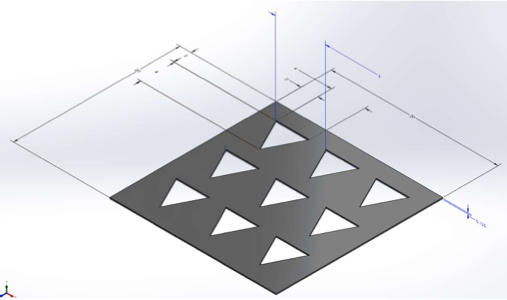
\includegraphics[width=0.8\textwidth]{../figs/introduction/thin_flat_mesh_design_with_cutouts.png}
        \caption{Refined thin mesh design with directional cutouts~\cite{RefWorks:RefID:371-bakhtardesign}.}
        \label{fig:introduction:initialThinMeshDesign}
\end{figure}

\paragraph*{Surface Texture\label{introduction:priorWork:otherTeamWork:deviceDesign:surfaceTexture}}

The mesh design needed to be fixed in place to address the concern of migration seen by existing devices like fiducial clips~\cite{RefWorks:RefID:344-mitchell2019adaptable}. The initial capstone team planned to secure the mesh to the tumor bed walls via suturing, though this could increase the implementation time substantially~\cite{RefWorks:RefID:372-krakovskytumor}. To address this adhesion concern, a texture was added to the top of the flat mesh to grab onto and increase friction between the mesh and tissue. Using the SolidWorks built in "Treadplate Bump" feature, a 3 x 3 mm treadplate bump with a texture offset of 0.75 mm and maximum element size of 0.125 mm was applied to the initial mesh~\cite{RefWorks:RefID:371-bakhtardesign}. This is shown below in Figure~\ref{fig:introduction:meshWithTreadplate}.

\begin{figure}[h!]
        \centering
        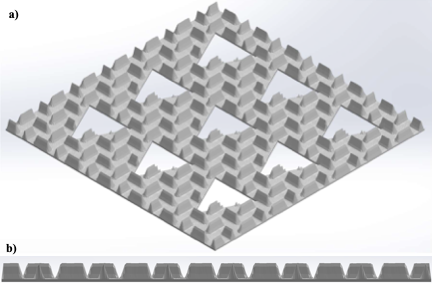
\includegraphics[width=0.8\textwidth]{../figs/introduction/mesh_design_with_treadplate.png}
        \caption{Isometric (a) and front view (b) of thin mesh design with treadplate bump appliedRefined thin mesh design with directional cutouts~\cite{RefWorks:RefID:371-bakhtardesign}.}
        \label{fig:introduction:meshWithTreadplate}
\end{figure}

\paragraph*{Friction and Implantation Testing\label{introduction:priorWork:otherTeamWork:deviceDesign:frictionTesting}}
To test the efficacy of the added surface texture, a friction test was performed. This test evaluated various texture and mesh geometry settings. The friction testing helped inform the device design by illustrating that a higher offset height and larger treadplate features yielded a higher static coefficient of friction.

The mock implantation testing, performed using raw chicken breast, showed that the textured mesh adhered closely to the cavity walls following excessive force and handling of the chicken breast. Both of these test setups are illustrated below in Figure~\ref{fig:introduction:frictionAndImplantationTesting}.

\begin{figure}[h!]
        \centering
        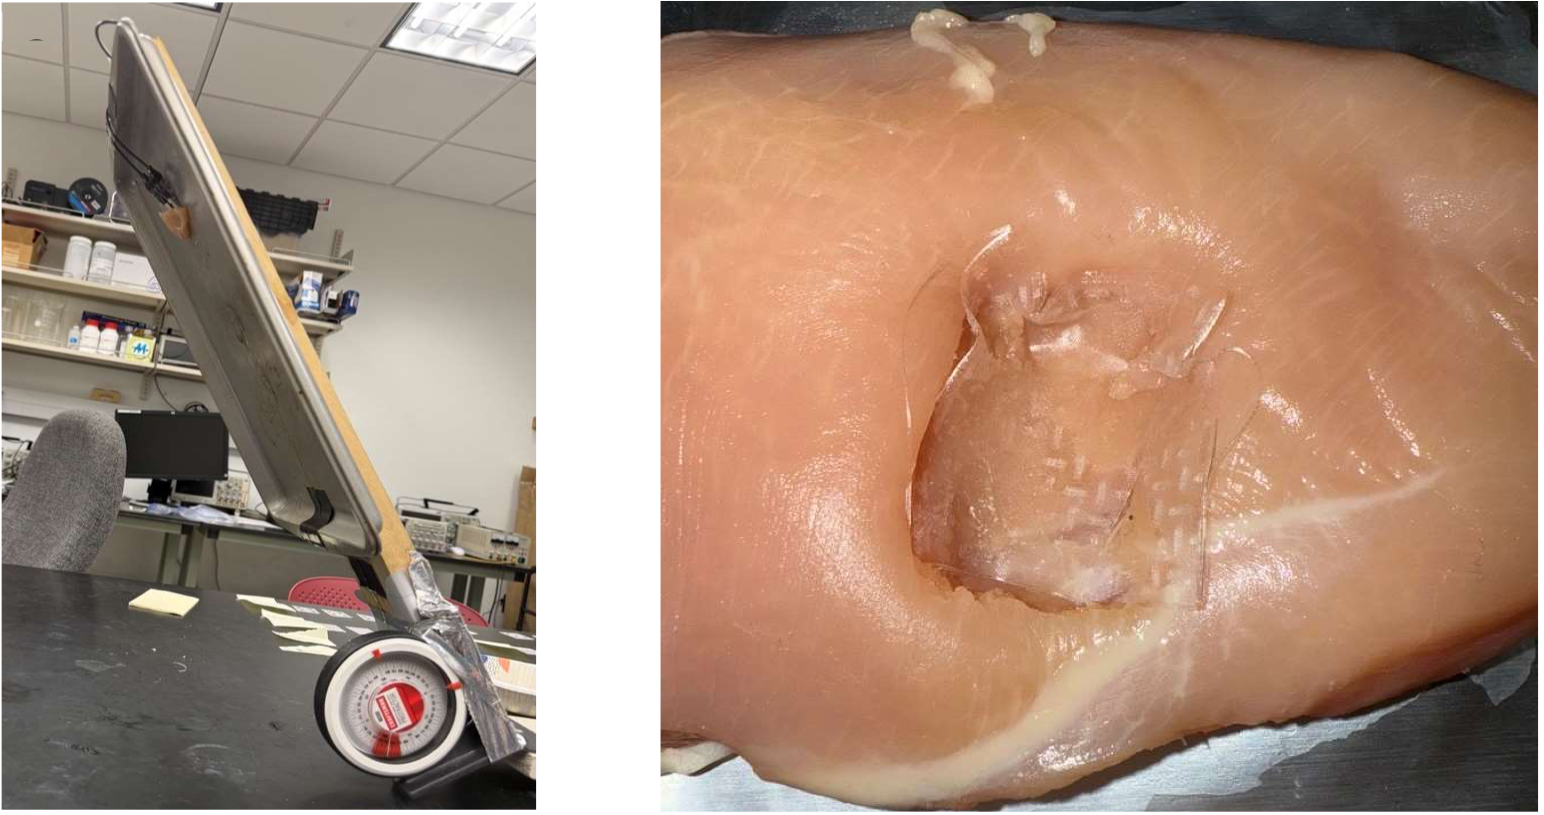
\includegraphics[width=0.8\textwidth]{../figs/introduction/friction_and_implantation_testing.png}
        \caption{Friction testing (left) and implantation testing (right)~\cite{RefWorks:RefID:371-bakhtardesign}.}
        \label{fig:introduction:frictionAndImplantationTesting}
\end{figure}

\subsubsection{Biodegradability Evaluation\label{sec:introduction:priorWork:otherTeamWork:biodegradabilityEval}}

Expanding on the capstone team's initial testing, a long-term biodegradability test was performed on the base material, PLCL. This degradation study used thin mesh squares to evaluate degradation timeline between 1 and 7 months at 37\textdegree C. While this study is still ongoing, one-month results showed an average mass loss of 0.071$\frac{gram}{month}$~\cite{RefWorks:RefID:371-bakhtardesign}.

\subsubsection{Initial Imaging Testing}

To help inform the device design, specifically the internal printing parameters of the device, initial imaging testing was performed on PLCL, PCL, PLA, and PLGA-HA filaments. The effects on radiopacity of infill density, infill pattern, sample height, and sample composition were evaluated through this imaging study.

It was found that PLCL, PCL, and PLA were essentially indistinguishable from one another, while PLGA-HA was marginally brighter. Limitations on this study resulted from the size of samples and subsequent resolution of results. In the future, larger samples may help draw clearer radiopacity conclusions~\cite{RefWorks:RefID:371-bakhtardesign}.

\subsubsection{Finite Element Modeling (FEM)\label{sec:introduction:priorWork:otherTeamWork:FEM}}

One researcher on the team, Zuhaib Jama, focused primarily on finite element modeling (FEM) as it pertained to the development of this new device. Three models were generated to evaluate the effects of line thickness on deformation, and it was found that a thickness of 0.5mm best matched the soft and ductile characteristics of breast tissue. Adipose tissue and glandular tissue were also evaluated using normal forces experienced during mamographies (49 to 186 N) to determine how much deformation the device may experience. Since adipose is softer than glandular tissue, the deformation and stresses found through this modeling represented the lower and upper bounds of deformation respectively~\cite{RefWorks:RefID:384-jamacomputational}. Visuals of this modeling are shown below in Figure~\ref{fig:introduction:femTesting}.

\begin{figure}[h!]
        \centering
        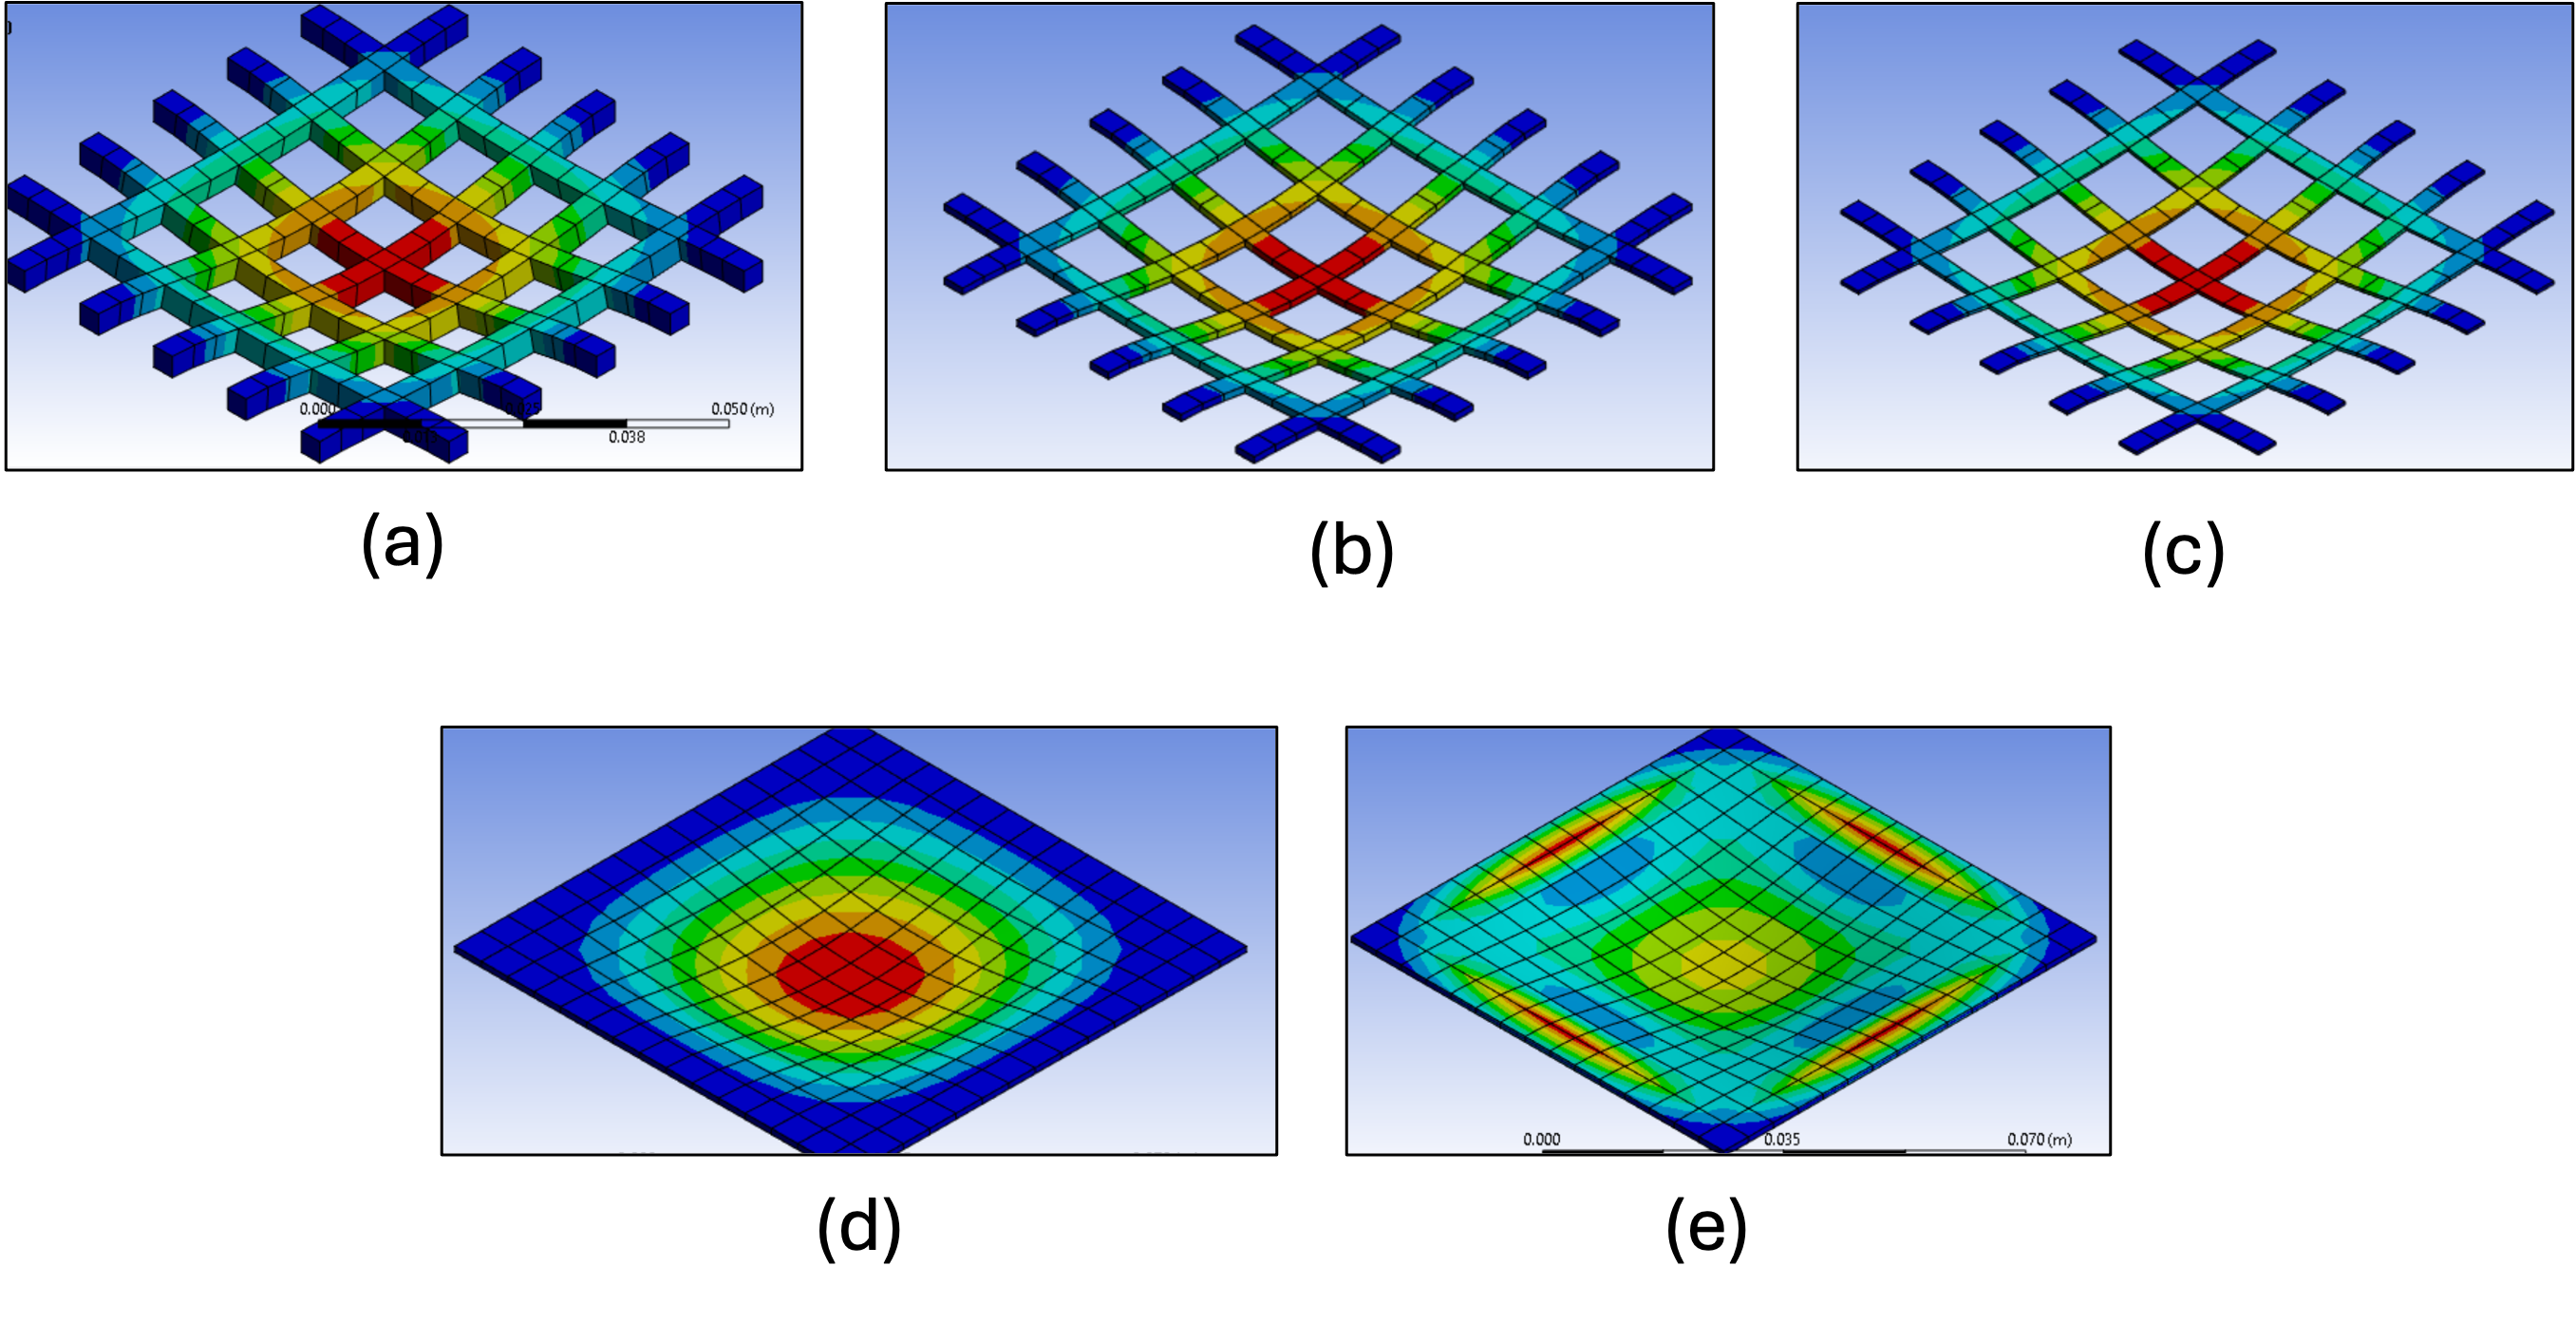
\includegraphics[width=0.8\textwidth]{../figs/introduction/fem_testing.png}
        \caption{FEM Modeling evaluating segment thickness (a-c, 3.175mm to 0.5mm) and properties of glandular (d) and adipose (e) tissue~\cite{RefWorks:RefID:384-jamacomputational}.}
        \label{fig:introduction:femTesting}
\end{figure}

\subsubsection{Initial PLCL Extrusions\label{sec:introduction:priorWork:otherTeamWork:plclExtrusions}}
% Trying to extrude a powder unsuccessfully
Initial extrusion testing was conducted on a Felfil EVO and Filabot EX6. Nomisma 70/30 PLCL powder was used for this extrusion testing~\cite{RefWorks:RefID:387-nomisma}. These two tabletop extruder systems are shown below in Figure~\ref{fig:introduction:felfilAndFilabotExtruders}.

\begin{figure}[h!]
        \centering
        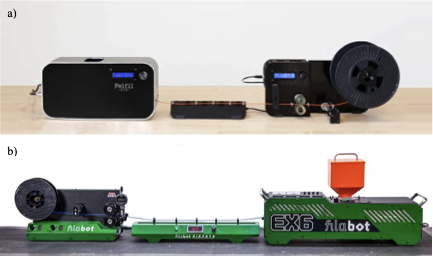
\includegraphics[width=0.8\textwidth]{../figs/introduction/felfil_and_filabot_extruders.png}
        \caption{Felfil Evo extruder and spooler setup (a) and Filabot EX6 extruder and spooler setup (b)~\cite{RefWorks:RefID:371-bakhtardesign}.}
        \label{fig:introduction:felfilAndFilabotExtruders}
\end{figure}

Both systems presented inconsistent flow speeds, severe diameter fluctuations, and yielded extremely brittle filaments. Drying the powder and filaments did not help with brittleness. It was determined that powder extrusions would require substantial additional research and development to yield printable filament~\cite{RefWorks:RefID:371-bakhtardesign}.

\subsection{Undergraduate Thesis\label{sec:introduction:priorWork:undergradThesis}}
The author defended an undergraduate thesis on the early stage development of this research in 2024. This thesis explored the mechanical properties of externally sourced PLCL filament to eventually compare to custom-made PLCL filament~\cite{RefWorks:RefID:370-einsteinisaac}~\cite{RefWorks:RefID:42-latticemedical}.

\subsubsection{Mechanical Testing of Lattice PLCL Filaments\label{sec:introduction:priorWork:undergradThesis:mechTesting}}

\paragraph*{Tensile Strength\label{sec:introduction:priorWork:undergradThesis:mechTesting:tensileStrength}}

To determine the tensile strength of the 3D printable material, a tensile test was performed following ASTM D638-14~\cite{RefWorks:RefID:4-test}. Given the scarcity and cost of the externally sourced filament, a Type V test specimen was used to frugally use materials.

Testing was performed at the Center for Design and Manufacturing Excellence (CDME) at Ohio State University on an Instron 5859 Universal Testing System.

Through testing of five specimen, it was found that the Lattice PLCL had an average Modulus of Elasticity of 20.929 MPA and an average Yield Strength of 17.361 MPa. The results of this experiment are shown below in Table~\ref{tab:introduction:undergradThesis:tensileTestResults}.

\begin{table}[H]
        \centering
        \caption{Results of Lattice PLCL Tensile Testing}
        \label{tab:introduction:undergradThesis:tensileTestResults}
        \begin{tabular}{lcc}
                \hline
                \textbf{Specimen Number}    & \textbf{Modulus of Elasticity (MPa)} & \textbf{Yield Strength (MPa)} \\
                \hline
                1                           & 22.720                               & 17.171                        \\
                2                           & 18.042                               & 15.935                        \\
                3                           & 20.465                               & 18.596                        \\
                4                           & 20.250                               & 15.820                        \\
                5                           & 23.170                               & 19.283                        \\
                \hline
                \textbf{Average}            & 20.929                               & 17.361                        \\
                \textbf{Standard Deviation} & 2.076                                & 1.554                         \\
                \hline
        \end{tabular}
        \label{tab:mechanical_properties}
\end{table}
% a. Tensile Strength
% b. Flexural Modulus
